\documentclass[11pt, oneside]{article}   	% use "amsart" instead of "article" for AMSLaTeX format
\usepackage{geometry}                		% See geometry.pdf to learn the layout options. There are lots.
\geometry{letterpaper}                   		% ... or a4paper or a5paper or ... 
\usepackage{graphicx}				% Use pdf, png, jpg, or eps§ with pdflatex; use eps in DVI mode
								% TeX will automatically convert eps --> pdf in pdflatex		
\usepackage{amssymb}
\usepackage{amsmath}
\usepackage{parskip}
\usepackage{color}
\usepackage{hyperref}

\graphicspath{{/Users/telliott_admin/Dropbox/Tex/png/}}
% \begin{center} 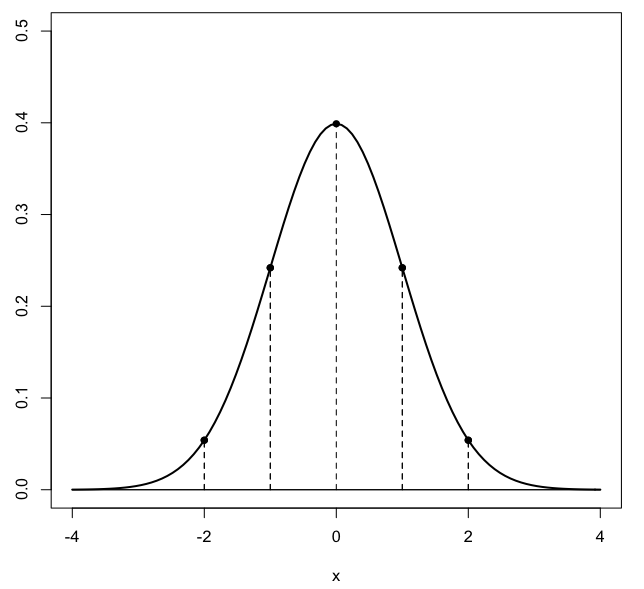
\includegraphics [scale=0.4] {gauss3.png} \end{center}

%break
\title{Fermat:  area under the exponential}
\date{}

\begin{document}
\maketitle
\Large

In computing Riemann sums, it isn't required that the intervals have the same width, only that the width of the largest goes to zero in the limit.

Courant and John describe a variation on Riemann sums using intervals of unequal (but graduated) width.  This "trick" allows them to derive the formula for
 
\[ \int x^n \ dx = \frac{x^{n+1}}{n+1} \]
\[ \int_a^b x^n \ dx = \frac{b^{n+1} - a^{n+1}}{n+1} \]
for all natural numbers $n$ first, and then with some elaborations, for real $n$ except $n = -1$.

This result (for integers) is due to Fermat and was achieved about 1640 (i.e. 25 years before Newton).  I found that proof on the web

\url{http://fredrickey.info/hm/CalcNotes/Fermat-Integration.pdf}

and there is also a good discussion in Maor's \emph{e, the Story of a Number}.  We'll look at Fermat's proof here and save the other for the Addendum (\hyperref[sec:Courant_Riemann]{\textbf{here}}). Fermat's version achieves simplicity by using the interval $[0,b]$ with its lower bound at zero.

\subsection*{derivation}

Let $E$ be a positive constant less than $1$.  Divide the region $[0,b]$ into subintervals with boundaries 
\[ \dots bE^3, \ bE^2, \ bE, \ b \]

How do we get the width of the largest rectangle to decrease to zero?  By taking the limit $E \rightarrow 1$.

Construct rectangles in the usual way that circumscribe the curve $y = x^n$ and add up their areas.  For the $i$th rectangle, the width is
\[ bE^i - bE^{i+1} \]
($bE^{i+1} < bE^i$), and the height is
\[ (bE^i)^n \]
so the overall sum is
\[ S = \sum_{i = 0}^{\infty} (bE^i)^n \ (bE^i - bE^{i+1}) \]
\[ = b^{n+1} \sum_{i = 0}^{\infty} (E^i)^n \ (E^i - E^{i+1}) \]
\[ = b^{n+1} \sum_{i = 0}^{\infty} (E^i)^{n+1} \ (1 - E) \]
\[ = b^{n+1} \ (1 - E) \ \sum_{i = 0}^{\infty} (E^{n+1})^i \]

Since $E$ is a positive constant less than $1$, $E^{n+1}$ is also.  Let $q = E^{n+1}$.  The sum becomes
\[ \sum_{i = 0}^{\infty} q^i = q^0 + q^1 + q^2 + q^3 + \dots \]
Recall that
\[ \frac{1}{1-x} = 1 + x + x^2 + x^3 + \dots \]
for $|x| < 1$.  

So, going back to $E$ we have
\[ S = b^{n+1} \ (1 - E) \ \frac{1}{1 - E^{n+1}} \]
and using the same identity again
\[ 1 - x = \frac{1}{1 + x + x^2 + x^3 + \dots } \]
so
\[ S = b^{n+1} \ \frac{1}{(1 + E + E^2 + E^3 + \dots)(1 - E^{n+1})} \]
All the terms in the infinite series starting at $E^{n+1}$ acquire counterparts with a minus sign, hence
\[ = b^{n+1} \ \frac{1}{1 + E + E^2 + E^3 + \dots + E^n} \]

Now take the limit as $E \rightarrow 1$.  The fraction becomes just
\[ \frac{1}{1 + E + E^2 + E^3 + \dots + E^n}  = \frac{1}{n+1} \]
and we have
\[ \int_0^b x^n = \frac{b^{n+1}}{n+1} \]
which is what we get when we evaluate $x^{n+1}$ on the interval $[0,b]$ and then divide by $n+1$.

This diagram from Maor uses slightly different nomenclature --- the interval points are of the form $a, ar, ar^2 \dots$ (moving from right to left).

\begin{center} 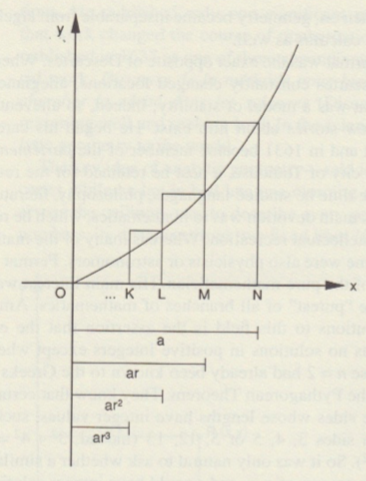
\includegraphics [scale=0.4] {Fermat_area1.png} \end{center}

\subsection*{Saint Vincent}

It turns out that the above analysis applies for integer $n < -1$, 

All except for the most important case, the hyperbola with $n = -1$.  The problem that we run into is division by zero.

However, a Belgian Jesuit named Saint Vincent noticed something about the intervals underneath the curve $y = 1/x$.  This work was completed about 1631 and published in 1647.

Starting at $N$ and moving backward, let's compute the width ($h$), height $h$ and area $A$ for each interval.

\begin{center} 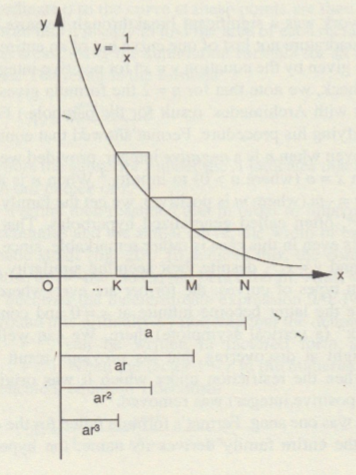
\includegraphics [scale=0.4] {Fermat_area2.png} \end{center}

N:
\[ w = a - ar = a(1-r), \ \ \ \  h = \frac{1}{a}, \ \ \ \ A = 1-r \]
M:
\[ w = ar - ar^2 = ar(1-r), \ \ \ \  h = \frac{1}{ar}, \ \ \ \ A = 1-r \]
L:
\[ w = ar^2 - ar^3 = ar^2(1-r), \ \ \ \  h = \frac{1}{ar^2}, \ \ \ \ A = 1-r \]

Maor:
\begin{quote}
This means that as the distance from 0 grows geometrically, the corresponding areas grow in equal increments, that is, arithmetically, and this remains true even when we go to the limit ...  But this in term implies that the relationship between area and distance is logarithmic.
\end{quote}

\textbf{The area under the curve 1/x is the logarithm}.  It took some time to figure out that the base of the logarithm was $e$.

\end{document}